\documentclass[]{article}
\usepackage{polyglossia}
\usepackage{fancyhdr}
\usepackage{enumerate}
\usepackage{framed}
\usepackage{listings}
\usepackage{amsfonts}
\usepackage[usenames,dvipsnames,svgnames,table]{xcolor}
\usepackage{minted}
\usepackage{hyperref}
\usepackage{graphicx}
\usepackage{gensymb}
\graphicspath{ {./images/} }

\setmainlanguage{spanish}
\definecolor{mygray}{RGB}{248,249,250}

\newcommand{\pythonblock}{\inputminted[linenos,bgcolor=mygray,framesep=10pt,firstnumber=\value{pythonnumber}]{python3}}
\newcommand{\asw}{\textbf{R. }}
\renewcommand{\theFancyVerbLine}{\sffamily \textcolor[rgb]{0.5,0.5,1.0}{\footnotesize \oldstylenums{\arabic{FancyVerbLine}}}}

\title{Evaluación Nº2 \protect\\ Algoritmos y programación}
\author{Anggelo Urso G. \\ anggelo.urso@inacapmail.cl}
\date{\today}

\pagestyle{fancy}
\fancyhf{}
\lhead{Algoritmos y programación}
\rhead{\thepage}
\lfoot{AUG /\LaTeX}
\rfoot{
\includegraphics[scale=0.4]{cc-lic}}

\hypersetup{
    colorlinks=true,
    linkcolor=blue,
    filecolor=magenta,      
    urlcolor=cyan,
}

\newcounter{pythonnumber}
\setcounter{pythonnumber}{1}

\begin{document}
    \thispagestyle{empty}
    \maketitle

    \section{Introducción}
    A continuación se entregan los detalles referentes a la evaluación 2 de la asignatura de algoritmos y programación. En el presente documento se detallara en cada una de las secciones y subsecciones los objetivos y detalles de ésta.

    A continuación se detallan los objetivos a ser alcanzados a través de la presente evaluación:

    \begin{itemize}
        \item Entrada y salida de datos.
        \item Sentencias de control de flujo:
        \begin{itemize}
            \item IF - ELSE - ELIF
            \item WHILE
            \item FOR-IN
        \end{itemize}
        \item Funciones
    \end{itemize}

    Se busca también que los alumnos perfeccionen su trabajo con la librería \textbf{math} y \textbf{turtle}, las cuales se busca el auto aprendizaje y la capacidad de búsqueda a través de la documentación adecuada.

    En la primera parte se detallará la descripción del problema, en donde se planteará el contexto del problema a ser resuelto. 

    En la segunda parte se detallará la descripción de la actividad, restricciones, figuras y objetivos a ser alcanzados con el desarrollo de la evaluación.

    Finalmente, se agregan las fechas y las formas de evaluación a ser consideradas para este trabajo.

    \section{Descripción del problema}
    La empresa constructora de Tony el Gordo, necesita un programa que permita planificar la construcción de una serie de edificios. 

    Esta planificación deberá entregar los costos y un diagrama de como quedarían los edificios a ser construidos por su empresa.

    Para esto se solicita a los alumnos entregar un programa (que utilice el módulo de \textbf{turtle}) para desplegar el gráfico.

    \section{Descripción de la actividad}
    \subsection{De las figuras a utilizar}
    Para llevar a cabo el gráfico, se utilizarán las siguiente figuras:

    \begin{itemize}
        \item Bloque de concreto (C): Deberá ser graficado como un cuadrado de tamaño 20 pasos.
        \item Bloque de vidrio (V): Deberá ser graficado como un cuadrado de tamaño 20 pasos, con una cruz en su interior.
        \item Bloque de techo (T): Deberá ser graficado como un triángulo equilátero de lado de 20 pasos.
        \item Debe existir una separación entre edificios de 10 pasos.
    \end{itemize}

    \subsection{De los costos de los bloques}
    Cada uno de los bloques tiene un costo específico. El coste se detalla en la siguiente tabla:\\

    \begin{center}
        \begin{tabular}{ |c|c| }
            \hline
            Tipo bloque & Valor \\
            \hline \hline
            Concreto & 40 \\
            \hline
            Vidrio & 60 \\
            \hline
            Techo & 30 \\
            \hline
        \end{tabular}
    \end{center}

    El costo del edificio corresponde a la suma de todos los bloques utilizados en la construcción de éste. Así por ejemplo un edificio que esté conformado por: \(C - V - V - C - T = 230 \)

    \subsection{De la entrada de los datos}
    Para la correcta planificación del edificio, el sistema solicitará, a través de entrada estándar (teclado), los materiales que serán utilizados para la confección de un edificio. Así, en el caso anterior tendríamos como entrada:\\

    \begin{minted}[linenos,bgcolor=mygray,framesep=10pt]{console}
> CCCVVCVT
> CCVVCVVCT
    \end{minted}

    Que corresponde al detalle de confección de dos edificios, con esto obtendremos como resultado de la entrada la siguiente figura:

    \begin{figure}[H]
        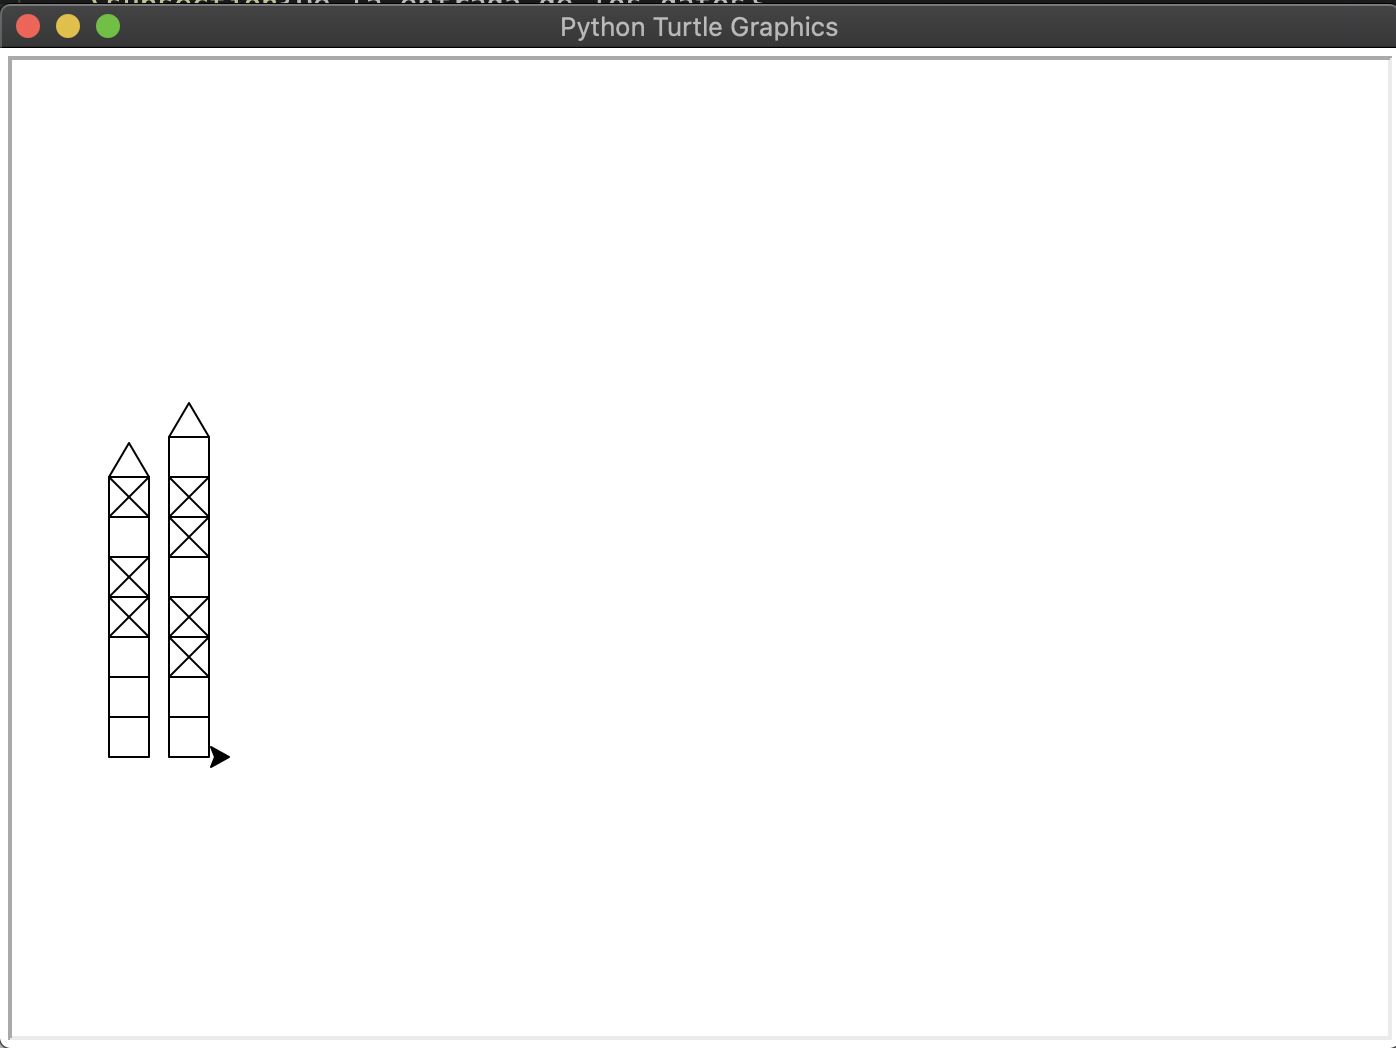
\includegraphics[scale=0.5]{first-input}
    \end{figure}

    Para finalizar la lectura de los edificios a ser creados, basta con ingresar un \textbf{enter} con una línea vacía y con eso debería cerrarse la lectura y entregar los resultados.\\

    \begin{minted}[linenos,bgcolor=mygray,framesep=10pt]{console}
> CCCVVCVT
> CCVVCVVCT
> 
    \end{minted}

    \subsection{De los resultados}
    Los resultados esperados para la evaluación del edificio, se espera que se entregue una respuesta similar a la que se presenta a continuación.\\

    \begin{minted}[linenos,bgcolor=mygray,framesep=10pt]{console}
> CCCVVCVT
> CCVVCVVCT
>

Total de edificios: 2
Costo total de edificio: 800

El costo del edificio 1 es: 370
El costo del edificio 2 es: 430
    \end{minted}

    Además de la interfaz del módulo de \textbf{turtle} en donde se aprecien los edificios dibujados.

    \subsection{Restricciones del problema}
    Como parte del entendimiento del problema, se establecen las siguientes restricciones:

    \begin{enumerate}
        \item No se puede comenzar el edificio con un vidrio (V).
        \item No se puede comenzar el edificio con el techo (T).
        \item No se puede tener sobre un bloque de techo (T), cualquier otro tipo de bloque. El edificio se termina con un techo.
        \item No se debe permitir el ingreso de un carácter inválido (los caracteres permitidos son V, T y C).
        \item Se deben validar los detalles de los materiales a ser utilizados para la confección del edificio \textbf{antes} de dibujarlo.
    \end{enumerate}

    \section{Detalle de la evaluación}
    La evaluación podrá ser realizada en parejas (máximo 2 personas), se espera que el comportamiento de la aplicación a ser desarrollada, sea similar al que se encuentra en el siguiente vídeo adjunto: \href{https://www.youtube.com/watch?v=Wle4ft3C88U}{https://www.youtube.com/watch?v=Wle4ft3C88U}.
    
    \subsection{Restricciones de la evaluación}
    Para la presente evaluación y en línea con los objetivos planteados inicialmente, se espera que los alumnos entreguen un trabajo con las siguientes restricciones:

    \begin{enumerate}
        \item Se deberá entregar un archivo fuente (formato \textbf{.py}) que permita ejecutar su programa.
        \item Se deberá respetar el formato de entrada de datos descrito en la sección anterior.
        \item Se deberá respetar el formato de salida de datos descrito en la sección anterior.
        \item Deberá contener a lo menos 3 funciones (1 por cada forma) y a lo menos 1 ciclo (para la entrada de datos).
        \item Deberán necesariamente utilizar la librería \textbf{turtle} y \textbf{math} para el desarrollo de su programa.
    \end{enumerate}

    \subsection{Ayudas con la interfaz}
    Como ayuda de la interfaz y que esta se adapte de forma correcta, deberán construir su programa agregando las siguientes líneas de código:\\

    \begin{minted}[linenos,bgcolor=mygray,framesep=10pt]{python}
from turtle import Turtle, Screen
from math import sqrt

screen = Screen()
screen.setup(700,500)

turtle = Turtle()
turtle.speed(100)
turtle.up()
turtle.goto(-300,-100)
turtle.down()

#sección de código
    \end{minted}

    Para agregar correctamente el carácter en el input, para recibir los datos del edificio pueden usar:\\

    \begin{minted}[linenos,bgcolor=mygray,framesep=10pt]{python}
edificio = input("> ")
    \end{minted}

    Así se rescatará la información de las partes que conforman el edificio, almacenándose dicho valor en la variable definida.

    \section{Fecha de entrega y formato}
    Se establece como fecha de entrega de la evaluación 2, el día domingo 19 de julio del 2020, antes de las 23:55 hrs.

    Solo será necesario que entreguen el archivo 1 de los miembros del equipo de trabajo, indicando a través de comentarios, claramente los integrantes de la siguiente manera:\\

    \begin{minted}[linenos,bgcolor=mygray,framesep=10pt]{python}
# Nombre apellido_paterno apellido_materno - RUT alumno 1
# Nombre apellido_paterno apellido_materno - RUT alumno 2
    \end{minted}
    
    En caso de ser solo un alumno se deberá respetar el mismo formato anterior en la cabecera del archivo, pero indicando los datos de un solo alumno.

    El formato de entrega será un archivo tipo Python (extensión \textbf{.py}) que deberá ser subido al ambiente de aprendizaje antes de la fecha indicada anteriormente.

    \textbf{Importante:} Bajo ningún punto se recibirán trabajos fuera de fecha o a través de otro medio que no sea el indicado anteriormente (AAI). Cualquier trabajo que se reciba en otro formato, otro medio o fuera de fecha \textbf{no será revisado}.
\end{document}